\fancyhead[L]{\textbf{\textsf{MỤC 1.5}}\quad \textsf{Hàm số ngược và hàm logarit}}
\fancyhead[R]{\textsf{\textbf{63}}}

\noindent
\begin{minipage}[t]{0.26\textwidth}
    \vspace{0pt}
    \centering
    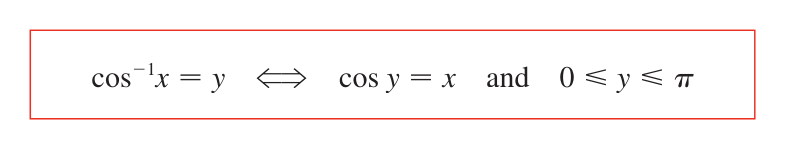
\includegraphics[width=\linewidth]{images/p0098_fig1.png}
    \vspace{-4pt}
    \begin{flushleft}
        \textbf{\textsf{HÌNH 21}}\\
        $y = \cos x,\ 0 \leqslant x \leqslant \pi$
    \end{flushleft}
    
    \vspace{1.8cm}
    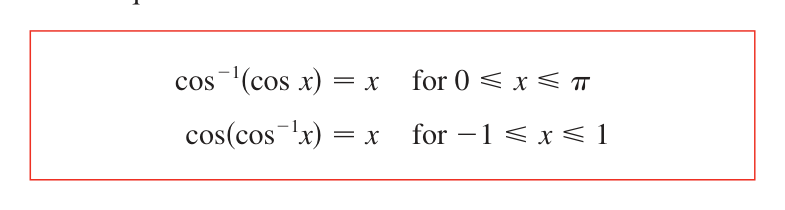
\includegraphics[width=\linewidth]{images/p0098_fig2.png}
    \vspace{-4pt}
    \begin{flushleft}
        \textbf{\textsf{HÌNH 22}}\\
        $y = \cos^{-1}x = \arccos x$
    \end{flushleft}
    
    \vspace{1.8cm}
    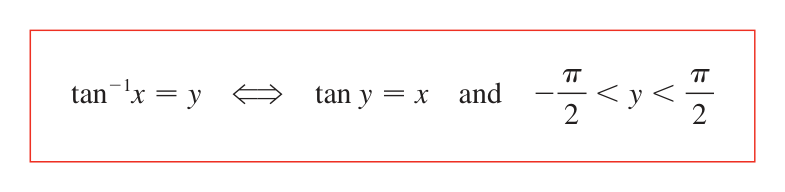
\includegraphics[width=\linewidth]{images/p0098_fig3.png}
    \vspace{-4pt}
    \begin{flushleft}
        \textbf{\textsf{HÌNH 23}}\\
        $y = \tan x,\ -\frac{\pi}{2} < x < \frac{\pi}{2}$
    \end{flushleft}
    
    \vspace{1.97cm}
    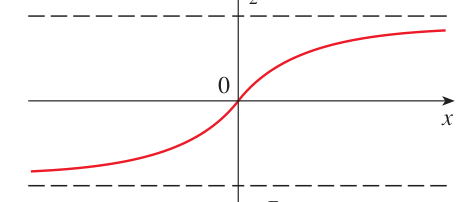
\includegraphics[width=\linewidth]{images/p0098_fig4.png}
    \vspace{-4pt}
    \begin{flushleft}
        \textbf{\textsf{HÌNH 24}}
    \end{flushleft}
\end{minipage}%
\hfill
\begin{minipage}[t]{0.71\textwidth}
    \vspace{0pt}
    \textbf{Hàm cosin ngược} được xử lý tương tự. Hàm cosin bị thu hẹp $f(x) = \cos x,\ 0 \leqslant x \leqslant \pi$, là hàm một-đối-một (xem Hình 21) và do đó nó có hàm ngược được ký hiệu là $\cos^{-1}$ hoặc $\arccos$.

    \vspace{0.16cm}
    \begin{tcolorbox}[colframe=stewartred, colback=white, sharp corners, boxrule=0.7pt, left=6pt, right=6pt, top=4pt, bottom=4pt]
        \[
        \cos^{-1}x = y \iff \cos y = x \quad \text{và} \quad 0 \leqslant y \leqslant \pi
        \]
    \end{tcolorbox}
    \vspace{0.08cm}

    Các phương trình triệt tiêu là
    
    \vspace{0.08cm}
    \begin{tcolorbox}[colframe=stewartred, colback=white, sharp corners, boxrule=0.7pt, left=6pt, right=6pt, top=4pt, bottom=4pt]
        \begin{align*}
        \cos^{-1}(\cos x) &= x \quad \text{với } 0 \leqslant x \leqslant \pi \\
        \cos(\cos^{-1}x) &= x \quad \text{với } -1 \leqslant x \leqslant 1
        \end{align*}
    \end{tcolorbox}
    \vspace{0.08cm}

    Hàm cosin ngược, $\cos^{-1}$, có tập xác định là $[-1, 1]$ và tập giá trị là $[0, \pi]$. Đồ thị của nó được minh họa trong Hình 22.

    Hàm tang có thể trở thành hàm một-đối-một bằng cách thu hẹp nó vào khoảng $(-\pi/2, \pi/2)$. Do đó \textbf{hàm tang ngược} được định nghĩa là hàm ngược của hàm số $f(x) = \tan x,\ -\pi/2 < x < \pi/2$. (Xem Hình 23.) Nó được ký hiệu là $\tan^{-1}$ hoặc $\arctan$.

    \vspace{0.16cm}
    \begin{tcolorbox}[colframe=stewartred, colback=white, sharp corners, boxrule=0.7pt, left=6pt, right=6pt, top=4pt, bottom=4pt]
        \[
        \tan^{-1}x = y \iff \tan y = x \quad \text{và} \quad -\frac{\pi}{2} < y < \frac{\pi}{2}
        \]
    \end{tcolorbox}
    \vspace{0.16cm}

    \noindent\textbf{\textsf{\color{stewartcyan}VÍ DỤ 14}}\quad Rút gọn biểu thức $\cos(\tan^{-1}x)$.

    \vspace{0.12cm}
    \noindent\textbf{\textsf{\color{stewartcyan}LỜI GIẢI 1}}\quad Đặt $y = \tan^{-1}x$. Khi đó $\tan y = x$ và $-\pi/2 < y < \pi/2$. Ta muốn tìm $\cos y$ nhưng vì đã biết $\tan y$, nên việc tìm $\sec y$ trước sẽ thuận tiện hơn:
    \begin{align*}
    \sec^2 y &= 1 + \tan^2 y = 1 + x^2 \\
    \sec y &= \sqrt{1 + x^2} \qquad {\color{stewartcyan}(\text{vì } \sec y > 0 \text{ với } -\pi/2 < y < \pi/2)}
    \end{align*}
    Do đó
    \[
    \cos(\tan^{-1}x) = \cos y = \frac{1}{\sec y} = \frac{1}{\sqrt{1 + x^2}}
    \]

    \noindent\textbf{\textsf{\color{stewartcyan}LỜI GIẢI 2}}\quad Thay vì dùng các đồng nhất thức lượng giác như trong Lời giải 1, sử dụng một hình học phẳng có lẽ trực quan hơn. Nếu đặt $y = \tan^{-1}x$, thì $\tan y = x$, và từ Hình 24 (minh họa cho trường hợp $y > 0$), ta suy ra được
    \[
    \cos(\tan^{-1}x) = \cos y = \frac{1}{\sqrt{1 + x^2}} \qquad\qquad {\color{stewartcyan}\blacksquare}
    \]

    \vspace{0.08cm}
    Hàm tang ngược, $\tan^{-1} = \arctan$, có tập xác định là $\mathbb{R}$ và tập giá trị là $(-\pi/2, \pi/2)$. Đồ thị của nó được biểu diễn trong Hình 25.

    \vspace{0.25cm}
    \noindent
    \begin{minipage}[b]{0.45\textwidth}
        \raggedleft
        \textbf{\textsf{HÌNH 25}}\\
        $y = \tan^{-1}x = \arctan x$
        \vspace{0.66cm}
    \end{minipage}%
    \hfill
    \begin{minipage}[b]{0.52\textwidth}
        \centering
        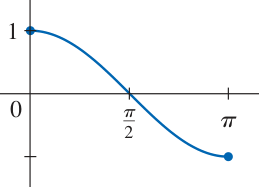
\includegraphics[width=\linewidth]{images/p0098_fig5.png}
    \end{minipage}
\end{minipage}